\section{Git Branches}
\begin{frame}[fragile]
  \slidetitle
  In this section we will learn to use git branches.
  In git the branches are not separated into different directories, but git rewrite the files when switching branches.
  Creating a new branch in git is cheap, git only creates a new file containing a hash pointing to the branch.
\end{frame}

\subsection{The master branch}
\begin{frame}[fragile]
  \subslidetitle

  The command \cmd{git branch} shows the branches:
  \begin{lstlisting}
(*\textcolor[HTML]{18B2B2}{(master)}*) $  (*\textcolor[HTML]{0000AA}{git branch}*)
* (*\textcolor[HTML]{00AA00}{master}*)
\end{lstlisting}

  The current branch is marked with an asterisk (*).
  \\
  \vspace{1em}
  Note: the default git branch is called \cmd{master}.

\end{frame}

\subsection{Creating branches}
\begin{frame}[fragile]
    \subslidetitle

To create a new \cmd{foo} branch, append the branch name to the \cmd{git branch} command.
\begin{lstlisting}
(*\textcolor[HTML]{18B2B2}{(master)}*) $ (*\textcolor[HTML]{0000AA}{git branch foo}*)
\end{lstlisting}

The \cmd{git branch} command lists you all your local branches
\begin{lstlisting}
(*\textcolor[HTML]{18B2B2}{(master)}*) $  (*\textcolor[HTML]{0000AA}{git branch}*)
  foo
* (*\textcolor[HTML]{00AA00}{master}*)
\end{lstlisting}

Note: the * character indicate which branch we are currently working on.
\end{frame}

\subsection{Switching to branch}
\begin{frame}[fragile]
    \subslidetitle
The \cmd{git checkout} command, is used to change the working branch.
\begin{lstlisting}
(*\textcolor[HTML]{18B2B2}{(master)}*) $ (*\textcolor[HTML]{0000AA}{git checkout foo}*)
Switched to branch 'foo'
(*\textcolor[HTML]{18B2B2}{(foo)}*) $ (*\textcolor[HTML]{0000AA}{git branch}*)
* (*\textcolor[HTML]{00AA00}{foo}*)
  master
\end{lstlisting}

The \cmd{git checkout} command with \cmd{-b} option creates a new branch and automatically switch to it.
\begin{lstlisting}
(*\textcolor[HTML]{18B2B2}{(foo)}*) $ (*\textcolor[HTML]{0000AA}{git checkout -b bar}*)
Switched to a new branch 'bar'
(*\textcolor[HTML]{18B2B2}{(bar)}*) $ (*\textcolor[HTML]{0000AA}{git branch}*)
* (*\textcolor[HTML]{00AA00}{bar}*)
  foo
  master
\end{lstlisting}
\end{frame}

\subsection{Deleting a branch}
\begin{frame}[fragile]
    \subslidetitle
To delete an existing branch use the \cmd{-d} or \cmd{-D} (force) flag:
\begin{lstlisting}
(*\textcolor[HTML]{18B2B2}{(bar)}*) $ (*\textcolor[HTML]{0000AA}{git checkout master}*)
(*\textcolor[HTML]{18B2B2}{(master)}*) $ (*\textcolor[HTML]{0000AA}{git branch foo bar -d}*)
Deleted branch foo (was c974445).
Deleted branch bar (was 9adadac).
(*\textcolor[HTML]{18B2B2}{(master)}*) $ (*\textcolor[HTML]{0000AA}{git branch}*)
* (*\textcolor[HTML]{00AA00}{master}*)
\end{lstlisting}

Note: you cannot delete the branch you are currently working on.

\end{frame}

% in general use diff to instruct changes

% create bugfix branch
\subsection{bugfix}
\begin{frame}[fragile]
    \subslidetitle

Our first bug report was filled out:
\newline \vspace{1em}
\#1: The title of the html page does not match the backgound

Start to create a new bugfix branch and implement the fix.
\begin{lstlisting}
(*\textcolor[HTML]{18B2B2}{(master)}*) $ (*\textcolor[HTML]{0000AA}{git checkout -b fix-title}*)
\end{lstlisting}

Modify the moon.html file following this diff instructions:
\begin{lstlisting}
diff --git a/moon.html b/moon.html
index 145cfff..ae7bc15 100644
--- a/moon.html
+++ b/moon.html
(*\textcolor[HTML]{18B2B2}{@@ -7,7 +7,8 @@}*)
         <style>
             body {
                 font-family: Monospace;
(*\textcolor{red}{-}*)                (*\textcolor{red}{background-color: \#f0f0f0; <!-- grey -->}*)
(*\textcolor[HTML]{00EE00}{+}*)                (*\textcolor[HTML]{00EE00}{background-color: black;}*)
(*\textcolor[HTML]{00EE00}{+}*)                (*\textcolor[HTML]{00EE00}{color: white;}*)
                 margin: 0px;
                 overflow: hidden;
             }
\end{lstlisting}
\end{frame}

% git diff master branch
\subsection{Display difference between branches}
\begin{frame}[fragile]
    \subslidetitle

As git has the complete history locally, we can easily display changes between branches:

\begin{lstlisting}
(*\textcolor[HTML]{18B2B2}{(fix-title)}*) $ (*\textcolor[HTML]{0000AA}{git diff master}*)
diff --git a/moon.html b/moon.html
index 145cfff..ae7bc15 100644
--- a/moon.html
+++ b/moon.html
(*\textcolor[HTML]{18B2B2}{@@ -7,7 +7,8 @@}*)
         <style>
             body {
                 font-family: Monospace;
(*\textcolor{red}{-}*)                (*\textcolor{red}{background-color: \#f0f0f0; <!-- grey -->}*)
(*\textcolor[HTML]{00EE00}{+}*)                (*\textcolor[HTML]{00EE00}{background-color: black;}*)
(*\textcolor[HTML]{00EE00}{+}*)                (*\textcolor[HTML]{00EE00}{color: white;}*)
                 margin: 0px;
                 overflow: hidden;
             }
\end{lstlisting}
\end{frame}

% display with tig/gitk
\subsection{Graphic display in tig}
\begin{frame}[fragile]
    \subslidetitle

Now we can see the graphical representation of our fix-title branch with tig
(*\textcolor[HTML]{18B2B2}{(fix-title)}*) $ (*\textcolor[HTML]{0000AA}{tig master fix-title}*)
\newline \vspace{1em}
  \centerline{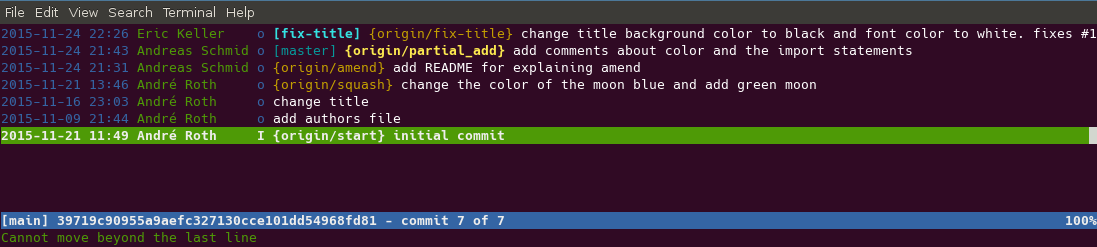
\includegraphics[width=10.5cm]{../screen/tig-fix-title.png}}
\end{frame}

% rebase with master
% display with tig/gitk
% create another feature branch
% 2 commits on this branch
% display with tig/gitk
% merge with master branch
% display with tig/gitk


% git checkout branch which was edited a long time ago, and we can continue to edit at this stage.


\subsection{git stash}
\begin{frame}[fragile]
    \subslidetitle
% clean, pop,
\end{frame}

\subsection{git diff}
\begin{frame}[fragile]
    \subslidetitle
\end{frame}

\subsection{Rebase a branch}
\begin{frame}[fragile]
    \subslidetitle
% -i
\end{frame}

\subsection{Merge a branch}
\begin{frame}[fragile]
    \subslidetitle
\end{frame}

\subsection{Rebase vs. Merge}
\begin{frame}[fragile]
    \subslidetitle
\end{frame}

\subsection{Cherrypick a commit}
\begin{frame}[fragile]
    \subslidetitle
\end{frame}

